%
%%% TERMINAL
%
\subsection{Terminal について}
\begin{frame}[containsverbatim]
\frametitle{Terminal の起動}
  \begin{itemize}
\item Launchpad からターミナルのアイコンをクリックして起動
\item これで shell が起動しファイル,ディレクトリの操作とプログラムの起動,終了ができます
  \end{itemize}
  \begin{center}
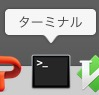
\includegraphics[scale=0.5]{./Figure/elementaryCS-figTermIcon.jpg}
  \end{center}
\end{frame}
\begin{frame}
\frametitle{ファイルに対する操作}
\scriptsize
  \begin{tabular}{l|l|lp{4cm}}
操作 & コマンド & 実行例 & \\\hline
生成 & touch & touch $name$ & 指定した名前で空のファイルを生成\\
名前変更 & mv & mv $oldfile\ newfile$ & $oldfile$ という名前を $newfile$ という名前に変更\\
複製 & cp & cp $srcfile\ dstfile$ & $srcfile$ を複製して $dstfile$ という名前をつける\\
表示 & less & less $name$ & $name$ の内容を表示\\
消去 & rm & rm $name$ & 指定した名前のファイルを消去
  \end{tabular}
\end{frame}
%\begin{frame}
%\frametitle{ディレクトリ}
%  \begin{itemize}
%\scriptsize
%\item ホームディレクトリはユーザアカウント毎にひとつ作られます
%\item ホームの下に適当なディレクトリを作成して管理してください
%\item 増えてきたら幾つかのグループに分けて管理すると便利です
%\item カレントディレクトリを目的のファイルがあるディレクトリまで移動して作業してください
%  \end{itemize}
%  \begin{center}
%\includegraphics[scale=.3]{../Figure/IL-figPath.eps}
%  \end{center}
%\end{frame}
\begin{frame}
\frametitle{ディレクトリに対する操作}
\scriptsize
  \begin{tabular}{l|l|lp{4cm}}
操作 & コマンド & 実行例 & \\\hline
作成 & mkdir & mkdir $name$ & 指定した名前で空のディレクトリを生成\\
一覧 & ls & ls $dir$ & $dir$ の中身一覧を表示\\
格納 & mv & mv $file\ dir$ & $file$ を消去して $dir$ に格納\\
     & cp & cp $file\ dir$ & $file$ を複製して $dir$ に格納\\
名称変更 & mv & mv $olddir\ newdir$ & $olddir$ を $newdir$ に変更\\
消去 & rmdir & rmdir $dir$ & 空の時には $dir$ を消去\\
     & rm    & rm -r $dir$ & 中身ごと $dir$ を消去\\
移動 & cd & cd $dir$ & 作業ディレクトリを移動\\
     & pushd & pushd $dir$ & 作業ディレクトリを移動して現在のディレクトリを保存\\
     & popd & popd $dir$ & 作業ディレクトリを保存したディレクトリに移動\\
表示 & pwd & pwd & 作業ディレクトリを表示\\
     & dirs & dirs & 保存したディレクトリを表示\\
  \end{tabular}
\end{frame}
\begin{frame}[fragile]
\frametitle{ターミナルをつかってみよう}
  \begin{itemize}
\item ターミナルを使って課題の準備をします
\item Terminal を起動
\item コマンドプロンプト \verb|>| が表示されたらホームディレクトリの下に適当なディレクトリ (ここでは CS1$\slash$kadai) を作成し
\item \href{https://sites.google.com/a/presystems.xyz/sample/home/elementary-computer-science}{\beamerbutton{https://sites.google.com/a/presystems.xyz/sample/home/elementary-computer-science}} から必要なファイルを作成したディレクトリにダウンロード
  \end{itemize}
  \begin{itembox}{課題準備}
\scriptsize
    \begin{verbatim}
> mkdir CS1/kadai # 課題用のディレクトリを作成
> cd CS1/kadai    # 課題用ディレクトリに移動
> cp sub-skeleton.py sub.py # 課題をコピー
    \end{verbatim}
  \end{itembox}
\end{frame}
%
%%% EDIT SROURCE FILE
%
\subsection{ソースファイルの編集}
\begin{frame}[containsverbatim]
\frametitle{ソースファイルの編集}
  \begin{itemize}
\item テキストエディタと呼ばれるソフトウェアを使って編集
    \begin{itemize}
\item vim, emacs など
    \end{itemize}
\item ターミナルからコマンド入力して起動
  \end{itemize}
  \begin{itembox}{editor の起動}
\scriptsize
    \begin{verbatim}
> open -a Macvim sub.py
あるいは
> open -a Emacs sub.py
    \end{verbatim}
  \end{itembox}
\end{frame}
%
%%% Run a Program
%
\subsection{プログラムを走らせてみる}
\begin{frame}[containsverbatim]
\frametitle{プログラムを走らせてみる}
  \begin{itemize}
\item コマンドプロンプト \verb|>| が表示されたら phtyon3 とソースファイル名と入力して return 
\item Python プログラムが実行されます
  \end{itemize}
  \begin{columns}
    \begin{column}{0.5\textwidth}
      \begin{itembox}{\footnotesize Python の起動}
\scriptsize
        \begin{verbatim}
> python3 sub.py
        \end{verbatim}
      \end{itembox}
    \end{column}
%    \begin{column}{0.5\textwidth}
%      \begin{itembox}{\footnotesize Ruby の起動と終了}
%\scriptsize
%        \begin{verbatim}
%> irb
%>> load smile.rb
%>> quit
%        \end{verbatim}
%      \end{itembox}
%    \end{column}
  \end{columns}
\end{frame}
